\documentclass[preprint,11pt]{elsarticle}
\usepackage[T1]{fontenc}\usepackage[utf8]{inputenc}\usepackage{lmodern}
\usepackage{amsmath,amssymb,amsthm,booktabs,graphicx,tabularx,multirow,array,xcolor}
\usepackage[ruled,vlined,linesnumbered]{algorithm2e}
\usepackage{microtype}\emergencystretch=3em\usepackage{verbatim}
\usepackage[hidelinks]{hyperref}
\usepackage{cleveref}
\usepackage{xr-hyper}


\journal{(journal to be chosen by the authors)}
% generated by code/experiments/aggregate.py -- do not edit
\newcommand{\ATwoK}{7}
\newcommand{\ATwoN}{7}
\newcommand{\AblNogpMedian}{2.7}
\newcommand{\AblPodonlyGt}{25\%}
\newcommand{\AblPodonlyShare}{75\%}
\newcommand{\BoneBand}{12\%}
\newcommand{\BoneBias}{1.08}
\newcommand{\BoneHi}{87\%}
\newcommand{\BoneK}{37}
\newcommand{\BoneLo}{63\%}
\newcommand{\BoneMedianAbs}{1.50}
\newcommand{\BoneN}{48}
\newcommand{\BoneOver}{4}
\newcommand{\BonePRaw}{0.18}
\newcommand{\BoneShare}{77\%}
\newcommand{\BoneShareSixtyfour}{92\%}
\newcommand{\BoneShareTwofiftysix}{62\%}
\newcommand{\BoneUnder}{7}
\newcommand{\BoneUnderTwofiftysix}{7}
\newcommand{\BoneVerdict}{met}
\newcommand{\BoneWithinTwofiftysix}{15}
\newcommand{\BtwoOneAcc}{100\%}
\newcommand{\BtwoOneActual}{18}
\newcommand{\BtwoOneMajor}{75\%}
\newcommand{\BtwoOneN}{24}
\newcommand{\BtwoOnePred}{18}
\newcommand{\BtwoOneVerdict}{met}
\newcommand{\BtwoTenthAcc}{88\%}
\newcommand{\BtwoTenthActual}{12}
\newcommand{\BtwoTenthMajor}{50\%}
\newcommand{\BtwoTenthN}{24}
\newcommand{\BtwoTenthP}{0.12}
\newcommand{\BtwoTenthPred}{15}
\newcommand{\BtwoTenthVerdict}{met}
\newcommand{\BudgetLsOne}{27}
\newcommand{\BudgetLsTen}{36}
\newcommand{\BudgetLsTenth}{19}
\newcommand{\BudgetMainLsTenth}{9}
\newcommand{\BudgetMainNlTenth}{4}
\newcommand{\BudgetNlOne}{28}
\newcommand{\BudgetNlTen}{36}
\newcommand{\BudgetNlTenth}{10}
\newcommand{\ClsLsAtFivetwelve}{12}
\newcommand{\ClsLsAtOnetwentyeight}{7}
\newcommand{\ClsLsAtSixtyfour}{8}
\newcommand{\ClsLsAtTentwentyfour}{13}
\newcommand{\ClsLsAtThirtytwo}{5}
\newcommand{\ClsLsAtTwofiftysix}{9}
\newcommand{\ClsNlAtFivetwelve}{5}
\newcommand{\ClsNlAtOnetwentyeight}{8}
\newcommand{\ClsNlAtSixtyfour}{5}
\newcommand{\ClsNlAtTentwentyfour}{8}
\newcommand{\ClsNlAtThirtytwo}{5}
\newcommand{\ClsNlAtTwofiftysix}{4}
\newcommand{\ClsTieAtFivetwelve}{7}
\newcommand{\ClsTieAtOnetwentyeight}{9}
\newcommand{\ClsTieAtSixtyfour}{11}
\newcommand{\ClsTieAtTentwentyfour}{3}
\newcommand{\ClsTieAtThirtytwo}{14}
\newcommand{\ClsTieAtTwofiftysix}{11}
\newcommand{\CoverMetCount}{5}
\newcommand{\CoverNotEvaluable}{0}
\newcommand{\CoverNotMetCount}{2}
\newcommand{\CpuDirectHi}{139}
\newcommand{\CpuDirectLo}{116}
\newcommand{\CpuGp}{44}
\newcommand{\CpuPodmlp}{86}
\newcommand{\DrawAgree}{83\%}
\newcommand{\DrawSign}{99\%}
\newcommand{\ExpBChanged}{15}
\newcommand{\ExpBImproved}{90\%}
\newcommand{\ExpBRetention}{88\%}
\newcommand{\ExpBShift}{0.24}
\newcommand{\ExpBTieToNn}{nine}
\newcommand{\ExpBTotal}{48}
\newcommand{\ExpFGain}{0.47}
\newcommand{\ExpFKept}{5}
\newcommand{\ExpFN}{7}
\newcommand{\ExtMedianExt}{$-$0.03}
\newcommand{\ExtMedianInterp}{0.16}
\newcommand{\FixedBestBetter}{12}
\newcommand{\FixedBestName}{\texttt{gp\_full[rbf]}}
\newcommand{\FixedBestRatio}{0.91}
\newcommand{\FixedBestRegret}{1.14}
\newcommand{\FixedBestShare}{75\%}
\newcommand{\FixedBestWorse}{two}
\newcommand{\FomMedianMs}{6.0}
\newcommand{\FomN}{36}
\newcommand{\FoneEvaluable}{yes}
\newcommand{\FoneFlagged}{15}
\newcommand{\FoneOk}{15}
\newcommand{\FoneShare}{100\%}
\newcommand{\FoneVerdict}{met}
\newcommand{\FullCellsN}{28}
\newcommand{\FullOverPod}{0.95}
\newcommand{\HfourAB}{10}
\newcommand{\HfourAC}{1}
\newcommand{\HfourAP}{0.006}
\newcommand{\HolmBOneSevenZero}{0.363}
\newcommand{\HolmSFourStrongWinsTwoFivepct}{0.630}
\newcommand{\HolmSOneShareLeTwoSevenFive}{0.003}
\newcommand{\HoneAMedian}{$-$0.059}
\newcommand{\HoneAP}{0.874}
\newcommand{\HoneBK}{5}
\newcommand{\HthreeCells}{five}
\newcommand{\HthreeFullJobs}{32}
\newcommand{\HthreeJobs}{15}
\newcommand{\HthreeProblems}{four}
\newcommand{\HthreeRecall}{47\%}
\newcommand{\HthreeSelected}{15}
\newcommand{\HtwoPHolm}{0.145}
\newcommand{\HwCores}{4}
\newcommand{\HwCpu}{Intel Xeon  @ 2.10GHz}
\newcommand{\IsoOverArd}{1.92}
\newcommand{\KrrNarrowN}{28}
\newcommand{\KrrNarrowRatio}{13}
\newcommand{\KrrNarrowShareThree}{18\%}
\newcommand{\KrrWideEightBeat}{61\%}
\newcommand{\KrrWideEightMed}{6.5}
\newcommand{\KrrWideEightShare}{21\%}
\newcommand{\KrrWideThirtytwoBeat}{64\%}
\newcommand{\KrrWideThirtytwoMed}{2.7}
\newcommand{\KrrWideThirtytwoShare}{57\%}
\newcommand{\LeakErrorRatio}{229}
\newcommand{\LeakMaxMatches}{0}
\newcommand{\LeakPlantedFlagged}{20}
\newcommand{\MetricAgreeMed}{95\%}
\newcommand{\NAllProblems}{44}
\newcommand{\NBenchTests}{56}
\newcommand{\NClassesOwn}{6}
\newcommand{\NHighP}{five}
\newcommand{\NMainProblems}{24}
\newcommand{\NOwnProblems}{36}
\newcommand{\NPerproblemRows}{44}
\newcommand{\NToolTests}{9}
\newcommand{\NTpProblems}{8}
\newcommand{\NTpTests}{6}
\newcommand{\NlClearTieBandZeroonefive}{6}
\newcommand{\NlClearTieBandZerothree}{3}
\newcommand{\NlClearTieBandZerozerofive}{10}
\newcommand{\NnFloorF}{$2.0\times10^{-4}$}
\newcommand{\NullRegret}{3.77}
\newcommand{\NullShare}{38\%}
\newcommand{\PLeFourLs}{20}
\newcommand{\PLeFourN}{30}
\newcommand{\PLeFourNl}{8}
\newcommand{\PlBoneHi}{90\%}
\newcommand{\PlBoneLo}{65\%}
\newcommand{\PlSoneHi}{1.01}
\newcommand{\PlSoneLo}{1.00}
\newcommand{\PlSoneWlo}{68\%}
\newcommand{\PlSthreeHi}{1.30}
\newcommand{\PlSthreeLo}{0.59}
\newcommand{\PlStwoHi}{0.98}
\newcommand{\PlStwoLo}{0.59}
\newcommand{\PlainAgree}{3}
\newcommand{\PlainN}{3}
\newcommand{\PlainOk}{3}
\newcommand{\PoneP}{0.18}
\newcommand{\PoneRho}{$-$0.38}
\newcommand{\PooledRmseBase}{1.07}
\newcommand{\PooledRmseCv}{0.62}
\newcommand{\PtwoGain}{0.60}
\newcommand{\PtwoPHolm}{0.051}
\newcommand{\RealRfourK}{9}
\newcommand{\RealRfourN}{12}
\newcommand{\RealRfourVerdict}{met}
\newcommand{\RealRoneMedian}{1.04}
\newcommand{\RealRoneVerdict}{met}
\newcommand{\RealRthreeK}{zero}
\newcommand{\RealRthreeVerdict}{met}
\newcommand{\RealRtwoK}{five}
\newcommand{\RealRtwoN}{six}
\newcommand{\RealRtwoVerdict}{met}
\newcommand{\RetroBetter}{12}
\newcommand{\RetroFlagged}{2}
\newcommand{\RetroGp}{0.93}
\newcommand{\RetroLeg}{1.00}
\newcommand{\RetroMax}{9.25}
\newcommand{\RetroMedian}{1.00}
\newcommand{\RetroN}{32}
\newcommand{\RetroShare}{97\%}
\newcommand{\RetroWorse}{7}
\newcommand{\RetroWorst}{\texttt{fisher\_L1} (9.2), \texttt{advdiff\_L1} (1.7), \texttt{helm\_L1} (1.1)}
\newcommand{\SeedAllLs}{80\%}
\newcommand{\SeedAllNl}{57\%}
\newcommand{\SfourBetter}{four}
\newcommand{\SfourMedian}{0.34}
\newcommand{\SfourN}{16}
\newcommand{\SfourStrongBetter}{4}
\newcommand{\SfourToolBetter}{11}
\newcommand{\SfourVerdict}{met}
\newcommand{\SfourWhi}{49\%}
\newcommand{\SfourWlo}{10\%}
\newcommand{\SoneCorrect}{6}
\newcommand{\SoneHi}{1.02}
\newcommand{\SoneLo}{1.00}
\newcommand{\SoneMax}{1.18}
\newcommand{\SoneMedian}{1.00}
\newcommand{\SoneMedianSixtyfour}{1.01}
\newcommand{\SoneMedianTentwentyfour}{1.00}
\newcommand{\SoneMedianTwofiftysix}{1.00}
\newcommand{\SoneN}{24}
\newcommand{\SonePRaw}{0.001}
\newcommand{\SoneShare}{100\%}
\newcommand{\SoneVerdict}{met}
\newcommand{\SoneWhi}{100\%}
\newcommand{\SoneWlo}{86\%}
\newcommand{\SthreeBetter}{11}
\newcommand{\SthreeHi}{1.19}
\newcommand{\SthreeLo}{0.59}
\newcommand{\SthreeLshapeRatio}{1.4}
\newcommand{\SthreeMaxRatio}{2.2}
\newcommand{\SthreeMaxWhere}{\texttt{heatcomp\_L2} at $N=1024$}
\newcommand{\SthreeMedian}{1.01}
\newcommand{\SthreeVerdict}{not met}
\newcommand{\SthreeWorse}{nine}
\newcommand{\StrongLegacyN}{15}
\newcommand{\StrongLegacyRatio}{0.64}
\newcommand{\StrongProblemsN}{two}
\newcommand{\StrongSecTentwentyfour}{429}
\newcommand{\StrongSecTwofiftysix}{146}
\newcommand{\StrongWorstProblemRatio}{152}
\newcommand{\StwoBetter}{15}
\newcommand{\StwoHi}{0.97}
\newcommand{\StwoLo}{0.59}
\newcommand{\StwoMedian}{0.85}
\newcommand{\StwoVerdict}{met}
\newcommand{\StwoWorse}{one}
\newcommand{\ToolFitSecSixtyfour}{7}
\newcommand{\ToolFitSecTentwentyfour}{312}
\newcommand{\ToolFitSecTwofiftysix}{112}
\newcommand{\ToolScaleRatio}{2.8}
\newcommand{\ToolTotalSecSixtyfour}{9}
\newcommand{\ToolTotalSecTentwentyfour}{426}
\newcommand{\ToolTotalSecTwofiftysix}{134}
\newcommand{\TpFomHi}{27}
\newcommand{\TpFomLo}{3}
\newcommand{\TpLsClear}{three}
\newcommand{\TpN}{eight}
\newcommand{\TpNotClear}{five}
\newcommand{\TpVerdict}{not met}
\newcommand{\VerNumpy}{2.5.3}
\newcommand{\VerOptuna}{5.0.0}
\newcommand{\VerPython}{3.13.16}
\newcommand{\VerScipy}{1.18.1}
\newcommand{\VerSkfem}{12.0.2}
\newcommand{\VerSklearn}{1.9.1}
\newcommand{\VerTorch}{2.14.1}

\begin{document}
\begin{frontmatter}
\title{Choosing a Fast Stand-In for a Slow Simulation: a Selection Tool and a \NAllProblems-Problem Study}
\author[a]{[Author names to be supplied by the authors]}
\address[a]{[Affiliations and corresponding-author e-mail to be supplied by the authors]}
\begin{abstract}
Engineers who depend on a slow simulation can afford only a limited number of runs, and must decide which fast stand-in model to train and whether more runs are worth the cost. We present SurroSelect, an open tool that chooses a stand-in from a pool of classical models by cross-validation, reports which models are tied, checks whether the POD basis limits accuracy, and forecasts the error for more runs. We tested it against criteria committed before the evaluation runs, on \NTpProblems{} problems solved by the third-party finite-element library \texttt{scikit-fem}, against a tuned neural network, and on two real measured datasets; a \NAllProblems-problem study describes where each model family wins. Selection was within a factor \SoneMax{} of the oracle (the best pool member by test error) in all \SoneN{} cells, although always choosing one full-field Gaussian process does almost as well. The error forecast for four times the budget was within a factor two in \BoneShare{} of \BoneN{} cases, but in only \BoneWithinTwofiftysix{} of 24 when starting from 256 runs. The tuned network beat the tool by more than 25\% in \SfourBetter{} of \SfourN{} cells, the limit of the criterion. The tool did not match the benchmark's own selection among methods that include networks, and the benchmark finding that a reduced-basis model wins at large budgets held on only \TpLsClear{} of the \TpN{} problems. All problems are simulated and their solvers are fast, so the tool's cost is justified only for much slower simulations.

\end{abstract}
\begin{keyword}surrogate model\sep Gaussian process\sep neural network\sep reduced-order model\sep parametric PDE\sep model selection\sep learning curve\end{keyword}
\end{frontmatter}
\section{Introduction}\label{sec:intro}
Many engineering decisions rest on a simulation that is too slow to run as often as one would like. Choosing the shape of a part, finding how uncertain an input leaves the answer, or fitting a model to measurements can each need thousands of runs. A common remedy is a \emph{surrogate}, or stand-in model: the simulation is run a limited number of times, say a few hundred, a cheap model is trained on the inputs and outputs, and the cheap model then replaces the simulation in all further work~\cite{quarteroni2016}. For example, if one run takes an hour, five hundred runs take about three weeks on one machine, whereas a trained stand-in answers in milliseconds.

The practical question is which kind of stand-in to build, and how many runs are enough. One long-standing route compresses the output fields with proper orthogonal decomposition (POD) and regresses the weights of the leading modes on the inputs, with a neural network~\cite{hesthaven2018,bhattacharya2021} or a Gaussian process~\cite{guo2018}. The other route trains a neural network to produce the whole field~\cite{fresca2022,franco2023}. Published comparisons are mixed. A survey of machine-learning solvers for fluid problems found that most papers claiming to beat a standard method used a weak baseline~\cite{mcgreivy2024}; kernel and Gaussian-process methods have been reported to be competitive with DeepONet~\cite{lu2021} and the Fourier neural operator~\cite{li2021} on benchmark problems~\cite{batlle2024}; and no universal winner was found between neural and polynomial surrogates~\cite{westermann2026}. A practitioner holding a few hundred runs of their own simulation still has no procedure that tells them which stand-in to use on \emph{their} data, how far it can be trusted, or how many more runs it would take to reach a target accuracy.

\paragraph{Gap} Existing comparisons rank methods on fixed problem sets and do not give the practitioner a validated procedure to select a stand-in, to see whether the POD basis limits accuracy, and to forecast the number of runs needed.

\subsection*{Motivation and contributions}
\begin{enumerate}
\item \textbf{A selection tool, SurroSelect} (Section 4). It fits a pool of stand-in models, chooses by cross-validation while reporting which models are tied with the best, checks whether the POD basis is the bottleneck, and forecasts the error for more runs from a learning curve. It is free software with a command-line interface (Sec.~S8).
\item \textbf{A pre-specified evaluation on problems solved by third-party code} (Section 6.3). Seven criteria were committed to version control before the evaluation runs on eight problems solved by the third-party finite-element library \texttt{scikit-fem} (smoke tests of the tool on three of them preceded the commit; see Section 7, limitation 2). We report which criteria were met and which were not, against a neural network tuned with a larger budget than any other method, and on two real measured datasets.
\item \textbf{A \NAllProblems-problem study of where each family wins} (Section 6.1, Section 6.2). Controls separate the effects of the reduced basis, of the regressor, and of how widely its hyper-parameters are searched, and the outcome of a comparison is shown to depend on the training budget and the tuning effort.
\item \textbf{A record of what did not work} (Section 7), including a pilot-data diagnostic that was not confirmed, a control that had to be widened after review, and every deviation from the plan (Supplement, Sec.~S4).
\end{enumerate}
The paper proposes no new regression model; the pool consists of classical methods, and the contribution is the procedure, its validation, and the evidence about when each member wins.

\subsection*{Organisation}
Section 2 reviews related work; Section 3 fixes notation and assumptions; Section 4 describes the method; Section 5 the experimental framework; Section 6 the results; Section 7 the discussion and limitations; Section 8 concludes.

\section{Related Work}\label{sec:related}
\subsection{Reduced-basis surrogates with learned coefficients}
Non-intrusive reduced-order models regress the weights of POD modes on the parameters. Hesthaven and Ubbiali used neural networks for this~\cite{hesthaven2018}, Bhattacharya et al.\ analysed PCA-based neural operators~\cite{bhattacharya2021}, and Guo and Hesthaven used Gaussian-process regression for nonlinear structural analysis~\cite{guo2018}. B\={e}rzi\c{n}\v{s} et al.\ compared radial-basis-function, Gaussian-process and neural-network regression inside one POD framework for extruder flows and reported several advantages of the Gaussian process~\cite{berzins2020}; we read only the abstract, and it is the closest precedent for our finding on smooth problems. Mora et al.\ proposed a hybrid Gaussian-process/neural operator framework~\cite{mora2025}.

\subsection{Neural networks, operators and nonlinear manifolds}
DeepONet~\cite{lu2021}, the Fourier neural operator~\cite{li2021} and the neural-operator framework~\cite{kovachki2023} learn maps between function spaces; autoencoders learn nonlinear latent manifolds for reduced models~\cite{lee2020,fresca2022,franco2023}. Our parameters are finite-dimensional, so we study direct and bottleneck networks rather than operator-input architectures. Whether a small linear basis can work depends on the decay of the Kolmogorov $n$-width~\cite{cohen2015}, which is slow for wave problems with discontinuous data~\cite{greif2019}.

\subsection{Kernel and Gaussian-process methods}
Gaussian processes are the standard low-dimensional regressor~\cite{rasmussen2006}. Batlle et al.\ develop a kernel framework with a priori error analysis and report it competitive with DeepONet and the Fourier neural operator~\cite{batlle2024}. A position paper argues that many neural-surrogate successes sit on low-dimensional manifolds where any competent reduced model interpolates well~\cite{duraisamy2026}.

\subsection{Fair comparison, tuning and reporting}
McGreivy and Hakim found that 79\% of 76 reviewed articles compared with weak baselines~\cite{mcgreivy2024}. De Hoop et al.\ study the cost--accuracy trade-off of neural architectures~\cite{dehoop2022}; Westermann et al.\ compare neural and polynomial surrogates by Pareto frontiers and find no universal winner~\cite{westermann2026}; a Common Task Framework has been proposed to evaluate scientific machine-learning methods against curated baselines~\cite{wyder2025}. Random search is an efficient alternative to grid search~\cite{bergstra2012}; adaptive early-stopping schemes such as Hyperband~\cite{li2018hyperband} and software such as Optuna~\cite{akiba2019} reduce tuning cost; reporting results as a function of tuning budget and accounting for run-to-run variance have been advocated~\cite{dodge2019,bouthillier2021}.

\subsection{Surrogate selection, learning curves and software}
Williams and Cremaschi compared eight surrogate forms on generated data to look for rules for choosing a form~\cite{williams2019}. Learning curves, the error as a function of training-set size, have been surveyed for decision making in supervised learning~\cite{mohr2024}, and error scaling laws have been fitted across data scales in deep learning~\cite{rosenfeld2020}. General-purpose libraries for model-order reduction~\cite{milk2016} and uncertainty quantification~\cite{marelli2014} exist; we did not compare their features with ours, and the finite-element library \texttt{scikit-fem}~\cite{gustafsson2020} is used here only to generate independent test problems. PDEBench~\cite{takamoto2022} provides large simulated benchmarks for scientific machine learning; we did not use it (Section 7).

\subsection{Comparison with prior work}
Table 1 lists what each closest work contains, judged from the parts we read (mostly abstracts; Westermann et al.\ in large part).
\begin{table}[t]\centering\caption{Closest related work. A dash means that we did not find the property in the parts we read (mostly abstracts); it does not prove absence.}\label{tab:related}\scriptsize\setlength{\tabcolsep}{2pt}\resizebox{\textwidth}{!}{\begin{tabular}{p{4.0cm}p{1.9cm}p{1.9cm}p{1.3cm}p{1.6cm}p{1.9cm}p{1.2cm}}
\toprule
Work & Kernel/GP vs neural & Tuning or baselines analysed & Ties reported & Selection guidance & Basis check, runs forecast & Open tool \\
\midrule
Hesthaven \& Ubbiali~\cite{hesthaven2018} & -- & -- & -- & -- & -- & -- \\
Guo \& Hesthaven~\cite{guo2018} & -- & -- & -- & -- & -- & -- \\
B\={e}rzi\c{n}\v{s} et al.~\cite{berzins2020} & \checkmark & -- & -- & -- & -- & -- \\
Batlle et al.~\cite{batlle2024} & \checkmark & -- & -- & -- & -- & -- \\
Westermann et al.~\cite{westermann2026} & \checkmark & -- & -- & -- & -- & -- \\
McGreivy \& Hakim~\cite{mcgreivy2024} & -- & \checkmark & -- & -- & -- & -- \\
Williams \& Cremaschi~\cite{williams2019} & -- & -- & -- & \checkmark & -- & -- \\
This paper & \checkmark & \checkmark & \checkmark & \checkmark & \checkmark & \checkmark \\
\bottomrule
\end{tabular}
}\end{table}

\subsection{Motivations}
(i) Method comparisons are reported on fixed problem sets, so a practitioner cannot tell whether a published ranking applies to their problem. (ii) The outcome of a comparison depends on tuning effort~\cite{mcgreivy2024,dodge2019}, so a tool must make the tuning effort explicit and equal. (iii) Small differences are often ties, so a tool should report ties instead of a single winner. (iv) The accuracy of any POD-based model is bounded by the basis (Proposition 2), which should be checked before tuning a regressor. (v) The practical question is the number of runs needed, which learning-curve extrapolation can answer only roughly and must be validated, not assumed.

\section{Preliminary Concepts}\label{sec:prelim}
\paragraph{Problem} A parametric simulation maps an input vector $\boldsymbol\mu\in[0,1]^p$ (rescaled to the unit box) to an output field $\mathbf u(\boldsymbol\mu)\in\mathbb R^m$ sampled on a fixed grid. We are given $N$ runs $\{(\boldsymbol\mu_i,\mathbf u_i)\}_{i=1}^N$ and want a model $\hat{\mathbf u}$ that is accurate on new inputs. Accuracy is the mean relative $L_2$ error over $n$ held-out inputs,
\begin{equation}\label{eq:err}
\mathrm{err}(\hat{\mathbf u})=\frac1n\sum_{j=1}^{n}\frac{\lVert\hat{\mathbf u}(\boldsymbol\mu_j)-\mathbf u(\boldsymbol\mu_j)\rVert_2}{\lVert\mathbf u(\boldsymbol\mu_j)\rVert_2}.
\end{equation}
\paragraph{POD basis} With $\bar{\mathbf u}$ the mean of the training fields and $V_r\in\mathbb R^{m\times r}$ the $r$ leading left singular vectors of the centred snapshot matrix, a POD model has the form
\begin{equation}\label{eq:pod}
\hat{\mathbf u}(\boldsymbol\mu)=\bar{\mathbf u}+V_r\,\hat{\mathbf a}(\boldsymbol\mu),
\end{equation}
where $\hat{\mathbf a}$ regresses the coefficients $\mathbf a=V_r^\top(\mathbf u-\bar{\mathbf u})$ on $\boldsymbol\mu$.
\paragraph{Regressors} \emph{Gaussian process (GP):} the posterior mean with a Mat\'ern-5/2 or squared-exponential kernel and one length-scale per input (ARD), hyper-parameters fitted by maximising the marginal likelihood~\cite{rasmussen2006}. \emph{Kernel ridge regression (KRR):} $\hat a(\boldsymbol\mu)=\sum_i\alpha_i k(\boldsymbol\mu,\boldsymbol\mu_i)$ with $\boldsymbol\alpha=(K+\lambda N I)^{-1}\mathbf a$. \emph{Polynomial:} ridge regression on total-degree monomials.
\paragraph{Ridge hat matrix and leave-one-out} For a ridge-type smoother the fitted values are $H\mathbf a$ with $H=K(K+\lambda N I)^{-1}$, and the leave-one-out residual of run $i$ is $(a_i-\hat a_i)/(1-H_{ii})$ (Proposition 1).
\paragraph{Tie band} Two errors are \emph{tied} if their ratio lies within $10^{\pm0.1}\approx1.26$; the outcome of a comparison of groups A and B is $\bar y=\log_{10}(\mathrm{err}_B/\mathrm{err}_A)$, positive when A is better, and a cell is a tie if $|\bar y|\le0.1$.
\paragraph{Assumptions}
\begin{description}
\item[A1] Inputs of training and test runs are drawn independently from the same distribution on the unit box; extrapolation tests (outside the box) are reported separately.
\item[A2] The output grid is the same for every run and the solver is deterministic (no noise).
\item[A3] Runs are exchangeable, so that $k$-fold cross-validation estimates the error on new runs. This fails for adaptive or clustered designs; the tool does not detect that.
\item[A4] The number of inputs is moderate (up to a few tens in our tests; only \NHighP{} of our \NAllProblems{} problems have ten or more).
\end{description}

\section{Proposed Methodology: SurroSelect}\label{sec:method}
\subsection{Overview}
SurroSelect takes the $N$ runs and returns (a) the selected stand-in, (b) the set of models tied with it, (c) a basis check, and (d) a learning-curve forecast (Fig. 1, Algorithm 1). Every step uses only the training runs.
\begin{figure}[t]\centering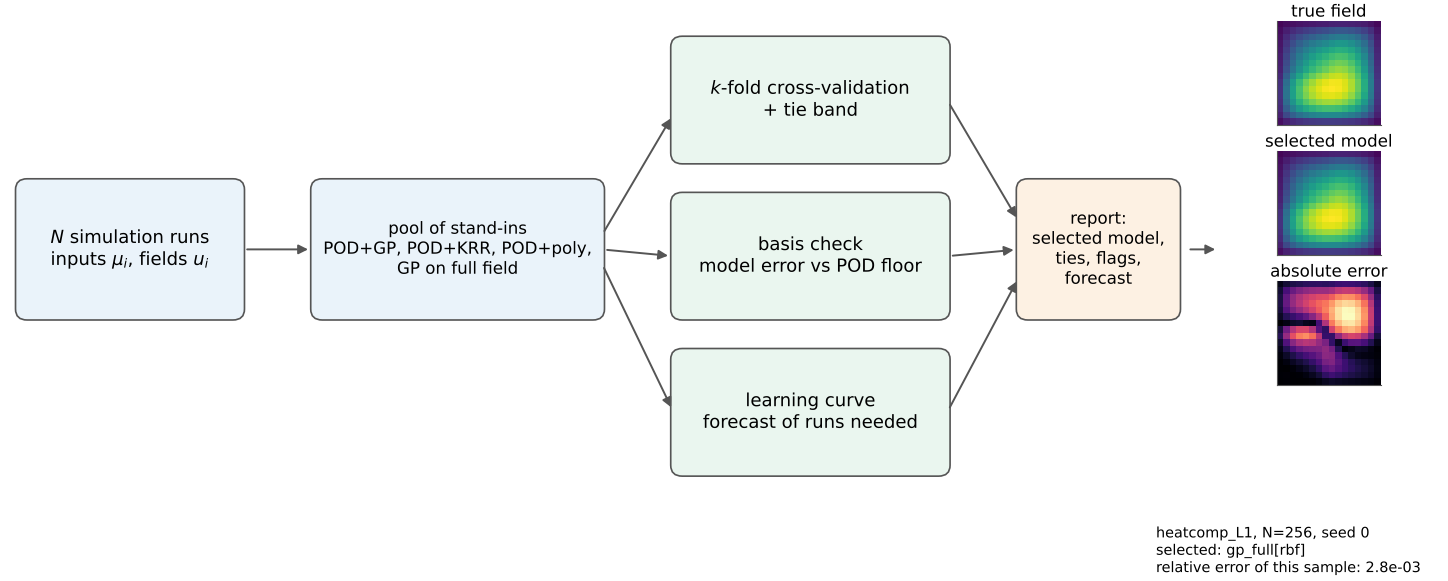
\includegraphics[width=\textwidth]{figures/fig_framework.png}
\caption{SurroSelect pipeline. The $N$ simulation runs enter a pool of stand-in models; $k$-fold cross-validation selects the best model and reports which others are tied with it; the basis check compares the model error with the error of projecting held-out fields onto the POD basis; the learning curve forecasts the error for more runs. The example fields are taken from the first test sample of problem \texttt{heatcomp\_L1} (seed~0, $N=256$): true field, selected model, and absolute error, as chosen by the rule in Section 6.5.}\label{fig:framework}\end{figure}

\subsection{Candidate pool}
The default pool has seven members, all classical: POD+GP with a Mat\'ern-5/2 kernel and rank 32, with a squared-exponential kernel and rank 32, and with Mat\'ern-5/2 and rank 8 (GP on the four leading modes with marginal-likelihood fitting, remaining modes sharing the fourth kernel); POD+KRR-wide, whose kernel, length-scale ($0.05$--$15\sqrt p$ on the unit box) and ridge ($10^{-16}$--$10^{-2}$ times $N$) are chosen over a wide grid by the leave-one-out error of Proposition 1; POD+polynomial, degree up to six with at most 3000 features, degree and ridge chosen by leave-one-out; and a GP directly on the full field (Mat\'ern-5/2 or squared-exponential, shared ARD kernel fitted on at most 300 runs), included only when $m\le2000$. A tuned neural network (\texttt{TunedMLP}, Section 5) can be added as an optional member.

\subsection{Cross-validated, tie-aware selection}
Each member is scored by $k$-fold cross-validation ($k=4$ by default) with all fitting, including hyper-parameter fitting, repeated inside each training fold. The member with the smallest mean cross-validated error~(1) is selected, and all members within the tie band of Section 3 are reported as tied. Members that fail to fit receive infinite error.

\subsection{Basis check}
On each fold, a rank-32 POD basis is fitted on the training part and the held-out fields are projected onto it; the mean relative error of this projection is the \emph{basis floor}. If the best POD-based member's cross-validated error is within 25\% of the floor, the tool flags the basis as limiting and recommends a full-field model, a larger basis, or a nonlinear output map. The reason is Proposition 2.

\subsection{Budget forecast}
For the selected member, cross-validated errors are computed at 1/8, 1/4, 1/2 and all of the training folds. A power law $e(n)=A\,n^{-b}$ is fitted by least squares in log--log coordinates to the last three points (central forecast) and to all four (alternative); the lower and upper of the two forecasts form a range. The number of runs needed for a target error $\varepsilon$ is $(A/\varepsilon)^{1/b}$; the tool declines to answer if $b<0.1$ or if the answer exceeds sixteen times the current number of runs. This is an extrapolation and is validated in Section 6.3, not assumed.

\begin{algorithm}\caption{SurroSelect (default settings)}\label{alg:surroselect}
\textbf{Input:} {runs $(\boldsymbol\mu_i,\mathbf u_i)_{i\le N}$, folds $k$, tie band $\tau=0.1$ decade, optional target error $\varepsilon$}
Scale inputs to the unit box; split the runs into $k$ folds\;
\textbf{for each} {pool member $c$}{ fit $c$ on each training fold and score it on the held-out fold; $e_c\leftarrow$ mean error (1)\;}
$c^\star\leftarrow\arg\min_c e_c$; tied set $\leftarrow\{c:\ e_c\le 10^{\tau}e_{c^\star}\}$; refit $c^\star$ on all $N$ runs\;
Basis floor $\phi\leftarrow$ mean projection error of held-out fields onto a rank-32 POD basis; flag the basis if $e_{c^\dagger}\le1.25\,\phi$ for the best POD-based $c^\dagger$\;
Learning curve: errors of $c^\star$ at $n\in\{N/8,N/4,N/2,N\}$ (training-fold sizes); fit $\log e=\log A-b\log n$ on the last three points (and on all four); forecast $e(4N)$; if $\varepsilon$ is given, return $(A/\varepsilon)^{1/b}$ unless $b<0.1$ or the result exceeds $16N$\;
\textbf{return} {$c^\star$, tied set, basis flag, forecast}
\end{algorithm}

\subsection{Theory}
Two results are standard and are included because the tool relies on them; proofs are in the Supplement (Sec.~S1).
\begin{proposition}[Closed-form leave-one-out]\label{prop:loo}
For a ridge smoother with hat matrix $H$ (so $\hat{\mathbf a}=H\mathbf a$ on the training inputs), the leave-one-out prediction error at run $i$ equals $(a_i-\hat a_i)/(1-H_{ii})$. For $H=K(K+\lambda N I)^{-1}$ with $K=Q\,\mathrm{diag}(w)Q^\top$, $1-H_{ii}=\sum_j Q_{ij}^2\,\lambda N/(w_j+\lambda N)$, which can be evaluated without cancellation when $\lambda N$ is tiny.
\end{proposition}
\begin{proposition}[Basis floor]\label{prop:floor}
Let $\hat{\mathbf u}$ be any model whose outputs lie in the affine subspace $\bar{\mathbf u}+\mathrm{span}(V_r)$. Then for every run, $\lVert\hat{\mathbf u}-\mathbf u\rVert_2\ge\lVert(I-V_rV_r^\top)(\mathbf u-\bar{\mathbf u})\rVert_2$, so the mean relative error of $\hat{\mathbf u}$ is at least the mean relative projection error of the basis, whatever the regressor.
\end{proposition}
The first is the PRESS identity for ridge regression~\cite{golub1979}; the second is the optimality of orthogonal projection. The forecast has no guarantee: it is exact only if the error follows a power law, and Section 6.3 tests how often it is useful.

\section{Experimental Framework}\label{sec:setup}
\subsection{Setup}
\paragraph{Data protocol} For each problem we generate 4096 candidate training inputs, 1000 held-out test inputs and 500 extrapolation inputs (coordinates drawn from $[-0.25,1.25]^p$, rejected if all lie inside the unit box) from streams seeded by the problem name; solutions are computed once and cached. A seed $s\in\{0,1,2\}$ fixes a permutation of the pool, and the training set for budget $N$ is its first $N$ elements, so training sets are nested within a seed. Budgets are $N\in\{32,\dots,1024\}$ for 24 problems and $\{64,256,1024\}$ for the others.
\paragraph{Problems} Table 2 lists the \NAllProblems{} problems. \NOwnProblems{} come from our own solvers, each verified against exact or manufactured solutions or by grid refinement; they are grouped into \NClassesOwn{} classes named after application areas (the classes are our own groupings of standard PDE families; nothing was calibrated to a real application). \NTpProblems{} problems were added in the final stage and solved with the independent finite-element library \texttt{scikit-fem} (version \VerSkfem); their unit tests compare with a series solution, a scaling law, load reversal, and mesh and time-step convergence. All data are simulated.
\begin{table}[t]\centering\caption{The \NAllProblems{} test problems by class. ``Inputs'' is the number of parameters $p$, ``Outputs'' the number of field values $m$.}\label{tab:problems}\small\resizebox{\textwidth}{!}{\begin{tabular}{lrrrl}
\toprule
Class & Problems & Inputs & Outputs & Solver \\
\midrule
Composite heat conduction & 2 & 4--9 & 256 & scikit-fem (third party) \\
Convection--diffusion & 2 & 3--4 & 256 & scikit-fem (third party) \\
Elastic L-shaped plate & 2 & 4--7 & 130 & scikit-fem (third party) \\
Transient heat, moving source & 2 & 3--5 & 192 & scikit-fem (third party) \\
Flow through porous rock & 9 & 3--32 & 256 & our code \\
Heat conduction & 9 & 3--8 & 128--256 & our code \\
Pollutant or heat carried by a flow & 4 & 4 & 128--256 & our code \\
Spreading fronts and reactions & 4 & 3--4 & 128--256 & our code \\
Thermal runaway & 2 & 3 & 256 & our code \\
Waves, shocks, acoustics & 8 & 3--4 & 128--256 & our code \\
\bottomrule
\end{tabular}
}\end{table}
\paragraph{Hardware and software} All runs used \HwCores{} CPU cores (\HwCpu), no GPU, Python \VerPython, NumPy \VerNumpy~\cite{harris2020}, SciPy \VerScipy~\cite{virtanen2020}, scikit-learn \VerSklearn~\cite{pedregosa2011}, PyTorch \VerTorch~\cite{paszke2019} and Optuna \VerOptuna~\cite{akiba2019}; each model fit used one thread.

\subsection{Metrics}
The error is (1). For outputs with a large offset (the real datasets, Section 6.6) the normalised root-mean-square error is used instead,
\begin{equation}\label{eq:nrmse}\mathrm{NRMSE}=\frac{\lVert Y-\hat Y\rVert_F}{\lVert Y-\bar Y_{\rm train}\rVert_F},\end{equation}
where $Y$ and $\hat Y$ stack the held-out true and predicted outputs and $\bar Y_{\rm train}$ is the mean of the training outputs. The comparison between a group A (here the reduced-basis group) and a group B (the direct networks) is
\begin{equation}\label{eq:y}\bar y=\frac1S\sum_{s=1}^S\log_{10}\frac{\mathrm{err}_B^{(s)}}{\mathrm{err}_A^{(s)}},\end{equation}
over seeds, with the best member of each group chosen on validation data; $\bar y>0.1$ means A is clearly better, $|\bar y|\le0.1$ is a tie. For the tool, the \emph{regret} of a cell $(q,N)$ (problem $q$, budget $N$) and the \emph{forecast ratio} of a case are
\begin{equation}\label{eq:regret}\mathrm{regret}(q,N)=\frac{\mathrm{err}(\text{selected})}{\min_{c\in\text{pool}}\mathrm{err}(c)},\qquad
\rho_{\rm forecast}=\frac{\hat e(4N_0)}{e_{\rm actual}(4N_0)},\end{equation}
with all errors measured on the 1000 test inputs; the actual error is that of the same pool member refit on $4N_0$ runs, and the forecast is within a factor two if $1/2\le\rho_{\rm forecast}\le2$. The \emph{reach-target classification} compares the statements $\hat e(1024)\le\varepsilon$ and $e_{\rm actual}(1024)\le\varepsilon$ for $\varepsilon\in\{1\%,0.1\%\}$ and reports the share of cases in which they agree, next to the share obtained by always giving the more common answer. Cell-wise values are geometric means over the three seeds.

\subsection{Baselines}
\begin{itemize}
\item \emph{The five-method benchmark} (``the benchmark'' below) under one tuning protocol: POD+GP, POD+polynomial, POD+MLP (reduced-basis group) and a direct MLP and a bottleneck MLP (network group). Each gets eight random-search trials (the first is a fixed default) scored on a random fifth of the training runs; networks use Adam for 1500 epochs in single precision.
\item \emph{Always POD+GP}: the benchmark's POD+GP, i.e.\ no selection; and \emph{the best fixed pool member}, the single member with the smallest median regret (identified after the fact, hence an optimistic reference).
\item \emph{Oracle}: the best pool member by test error (an upper bound; unavailable in practice).
\item \emph{Strongly tuned network}: \texttt{TunedMLP}: Optuna TPE with successive-halving pruning~\cite{akiba2019,li2018hyperband}, 16 trials over output type (full field or POD rank 8/16/32), depth 2--4, width 64--256, activation, learning rate and weight decay; full-batch float64 training; final refit on all runs with four times the epochs and 200 L-BFGS iterations. Compared with the benchmark networks it has about twice the number of trials, four times the epochs, double precision and an L-BFGS polish; it is selected on a validation split of the training runs only, and it was run only at $N=256$ and $1024$ (16 cells).
\end{itemize}
Controls for the mechanism study are described in Section 6.1.

\subsection{Hypotheses and how each is tested}
The hypotheses, metrics and pass/fail criteria below were committed to version control before the corresponding results (commit hashes in Supplement, Sec.~S2); Table 3 lists them. Earlier-stage hypotheses (pilot diagnostic, mechanism controls, longer training) are in the Supplement (Sec.~S3).
\begin{table}[t]\centering\caption{Pre-specified hypotheses for the tool and their pass criteria (cells: 8 problems $\times$ $N\in\{64,256,1024\}$ = 24).}\label{tab:hyp}\small
\begin{tabularx}{\textwidth}{lXX}\toprule ID & Statement & Pass criterion\\\midrule
H1a & Cross-validated selection is close to the oracle & median regret $\le1.5$ and $\ge75\%$ of cells $\le2$\\
H1b & Not worse than always using POD+GP & median ratio $\le1$\\
H1c & At least as good as the benchmark's own selection & median ratio $\le1$; more cells better than worse by $>10\%$\\
H2 & The forecast is usable & 4$N_0$ forecast within a factor 2 in $\ge70\%$ of 48 cases; reach-target classification $\ge75\%$\\
H3 & The basis flag identifies cases where a full-field model is better & $\ge75\%$ of flagged cells (if at least five)\\
H4 & A tuned network rarely beats the tool & better by $>25\%$ in at most 4 of 16 cells\\
H5 & The benchmark finding holds on problems solved by third-party code & at least 5 of 8 problems reduced-basis-clear at $N=1024$\\
\bottomrule\end{tabularx}\end{table}
Binomial proportions are given with Wilson 95\% intervals~\cite{wilson1927}; medians with percentile bootstrap intervals (2000 resamples over cells); the tests against the thresholds are one-sided exact binomial tests with Holm adjustment~\cite{holm1979} over the three that admit one.

\section{Results and Analysis}\label{sec:results}
All numbers in this section are written by the aggregation script from the result files. Cell-wise values are geometric means over three seeds; intervals are 95\%.

\subsection{Where each family wins, and by how much (the evidence base)}\label{sec:results-study}
\paragraph{Main problems} Fig. 2 shows the outcome $\bar y$ of (4) for the reduced-basis group against the direct networks. Among the \NMainProblems{} main problems (those with the full budget range), the reduced-basis group is clearly better in \ClsLsAtThirtytwo{} problems at $N=32$, the networks in \ClsNlAtThirtytwo{}, and \ClsTieAtThirtytwo{} are ties; at $N=1024$ the counts are \ClsLsAtTentwentyfour{}, \ClsNlAtTentwentyfour{} and \ClsTieAtTentwentyfour{}. The number of network wins at $N=1024$ is \NlClearTieBandZeroonefive{} if the tie band is widened to 0.15 decade and \NlClearTieBandZerozerofive{} if it is narrowed to 0.05, so counts of ties and small wins are not stable. Where the reduced basis wins, it can win by orders of magnitude (panel b, top rows); where networks win, the largest margin is a factor of about three.
\begin{figure}[t]\centering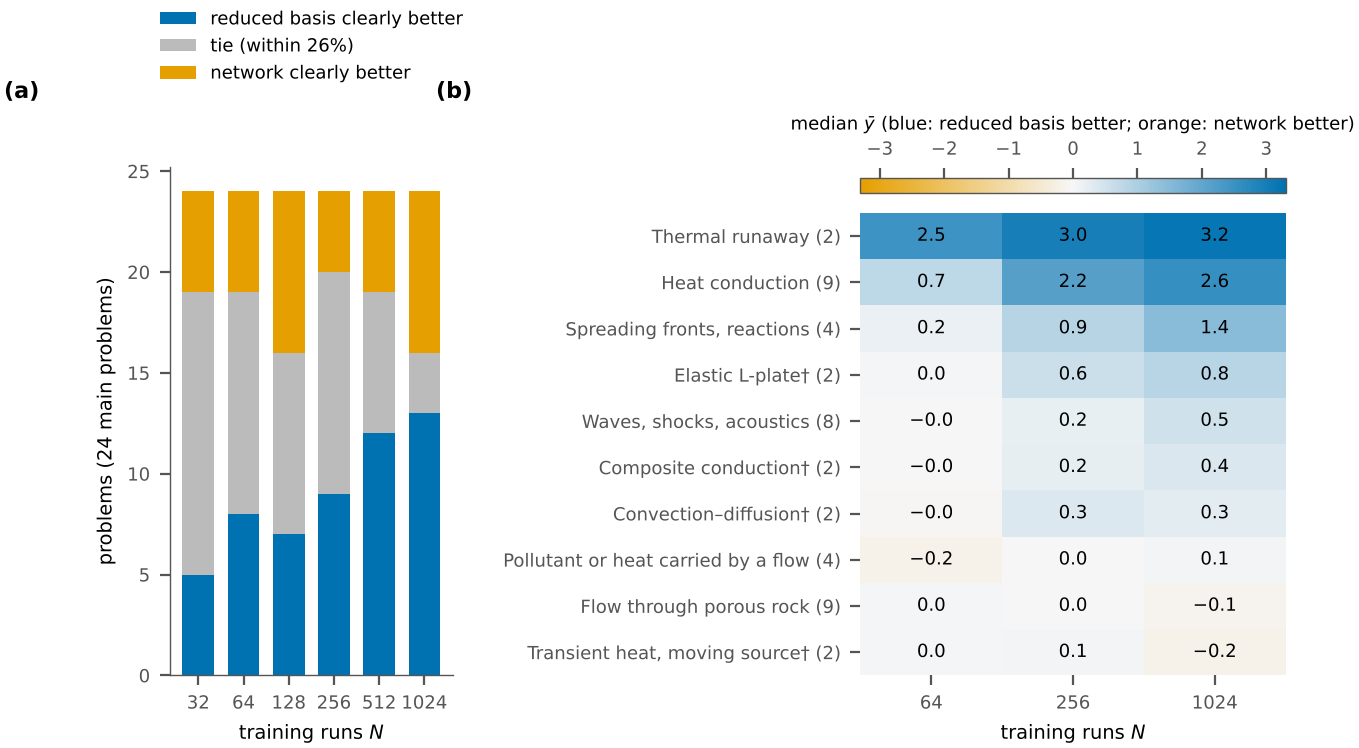
\includegraphics[width=\textwidth]{figures/fig_main_result.png}
\caption{The reduced-basis group wins clearly on smooth problems at large budgets, and most differences at small budgets are ties. (a) Number of the \NMainProblems{} main problems (own solvers; five methods; three seeds; tie band $\pm0.1$ decade) in which the reduced-basis group is clearly better, tied, or clearly worse than the direct networks, by training budget. (b) Median signed effect $\bar y$ by problem class over all \NAllProblems{} problems (number of problems in brackets; $\dagger$: solved with \texttt{scikit-fem}); the colour scale is centred at zero and blue is the same colour as in (a). Per-problem values are in Supplement Table~S3. The $N=1024$ results are confounded with a doubling of the networks' optimiser steps (Supplement Sec.~S3).}\label{fig:main}\end{figure}
\paragraph{Accuracy reached} For a coarse target of 10\% error, both groups reach it on all 36 own-solver problems within 1024 runs; for 1\% they are about equal (\BudgetLsOne{} against \BudgetNlOne{} problems); at the demanding end, 0.1\%, the reduced-basis group reaches it on \BudgetLsTenth{} problems and the networks on \BudgetNlTenth{} (\BudgetMainLsTenth{} against \BudgetMainNlTenth{} among the 24 main problems, excluding the eight smooth problems we added later because we expected the Gaussian process to do well). On our own problems a solve takes a median of \FomMedianMs{}~ms, so fitting a surrogate costs more than running the simulation 1024 times on most of them; the case for surrogates rests on simulations much slower than ours, and the comparison that matters is accuracy per run.
\paragraph{Problems solved by third-party code (H5)} On the eight problems solved by \texttt{scikit-fem}, the reduced-basis group is clearly better at $N=1024$ in \TpLsClear{} of \TpN{}; the criterion of at least five (H5) is therefore \textbf{\TpVerdict}. The other problems are ties or network wins (Table~S3): the networks are ahead on the composite-conduction problem with nine inputs and high contrast and on both moving-source problems. The simple picture ``reduced basis wins at large budgets'' therefore does not carry over to \TpNotClear{} of these \TpN{} problems; the tool of Section 4 is designed for exactly this case, and Section 6.3 tests it.

\subsection{Why the Gaussian-process reduced model wins when it does}\label{sec:results-mech}
Fig. 3 compares alternatives with the Gaussian-process reduced model in the \KrrNarrowN{} budget--problem combinations (budgets 64, 256, 1024) where it clearly beats the best network (the comparison uses the best network by \emph{test} error, an oracle that favours the networks). Kernel ridge with the narrow range of ridge and length-scale of our first control is a median \KrrNarrowRatio{} times less accurate; with a wide range and the same eight tuning trials, \KrrWideEightMed{} times; with 32 trials, \KrrWideThirtytwoMed{} times (\KrrWideThirtytwoShare{} of cells within a factor three), and the wide kernel ridge beats the best network clearly in \KrrWideThirtytwoBeat{} of these cells. A Gaussian process on the full field without POD is as accurate as the POD-based one (median ratio \FullOverPod). The Gaussian-process advantage is therefore largely an advantage of a smooth regressor whose regularisation is searched widely and finely, and not of the reduced basis; we did not isolate the contribution of marginal-likelihood fitting, because its cost is not matched by the kernel-ridge search. The wide-range control was added after an AI-agent review of an earlier draft showed that our first control could not reach the regularisation that near-interpolating fits need; this is a post hoc control (Supplement, Sec.~S2).
\begin{figure}[t]\centering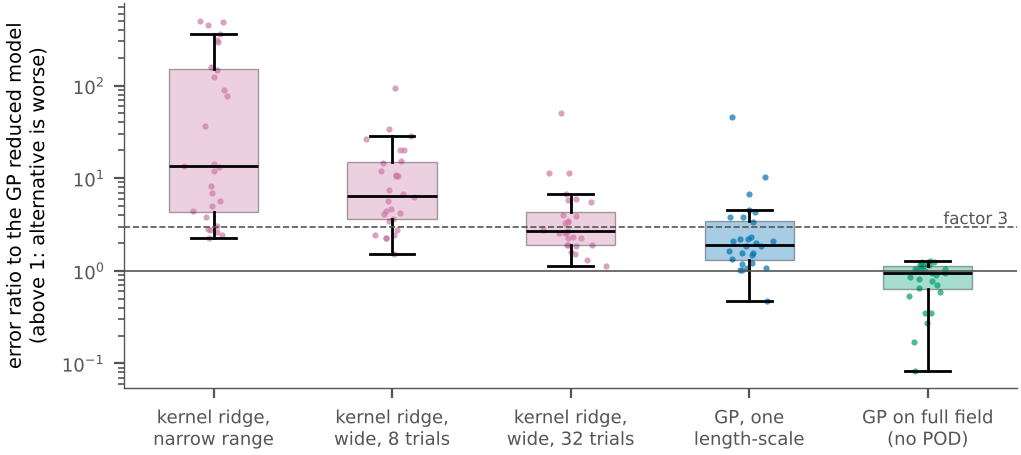
\includegraphics[width=0.85\textwidth]{figures/fig_mechanism.png}
\caption{Widening the hyper-parameter search of kernel ridge closes most of the gap to the Gaussian-process reduced model, and a Gaussian process on the full field is as good as the POD-based one. Error ratio of each alternative to the reduced-basis Gaussian process in the \KrrNarrowN{} budget--problem combinations where that model clearly beats the best network (own-solver problems, budgets 64, 256, 1024); boxes show quartiles, dots individual combinations, the dashed line a factor of three.}\label{fig:mech}\end{figure}
Three further results qualify the picture. Training the networks four times longer moved the verdict in \ExpBChanged{} of \ExpBTotal{} cases, always toward the networks, and improved \ExpBImproved{} of the refits; the large gaps survived stronger training (double precision, 6000 steps, L-BFGS) in \ExpFKept{} of \ExpFN{} decisive problems, with the networks' error floor lowered by a median \ExpFGain{} decade to about \NnFloorF. On the extrapolation test set the median $\bar y$ at $N=1024$ is \ExtMedianExt{} instead of \ExtMedianInterp{}. And the class of a cell agrees between halves of the random-search draws in \DrawAgree{} of cases (sign of clear differences: \DrawSign), so small differences should not be over-interpreted. The earlier-stage hypotheses, including the pilot diagnostic that was not confirmed, are in the Supplement (Sec.~S3).

\subsection{Evaluation of SurroSelect on problems solved by third-party code}\label{sec:results-tool}
The tool was run on the eight \texttt{scikit-fem} problems at $N\in\{64,256,1024\}$ with three seeds (24 cells), and every pool member was also refit and scored on the 1000 test inputs, so that the \emph{oracle} (the best pool member by test error; unavailable in practice) is known. Table 4 lists the pre-specified criteria and what was observed; Table 5 gives the errors per problem. Only eight problems from four families are involved, and the three seeds of a problem share the pool and the test set, so cells are not independent; Table 4 therefore also gives problem-level intervals (resampling the eight problems), and the verdicts describe these eight problems only. The tuned network was run only at $N=256$ and $1024$ (16 cells); Fig. 5 shows it next to the tool.
\begin{table}[t]\centering\caption{Pre-specified criteria (Table 3) and results on the eight problems solved by third-party code. Intervals are 95\% (bootstrap for medians, Wilson for proportions, both treating cells as independent); problem-level intervals are in the text. The Holm-adjusted $p$-values are one-sided exact binomial tests against the thresholds.}\label{tab:criteria}\footnotesize\resizebox{\textwidth}{!}{\begin{tabular}{p{1.5cm}p{4.4cm}p{5.2cm}p{1.3cm}p{1.6cm}}
\toprule
ID & Criterion & Observed (95\% interval) & Holm $p$ & Verdict \\
\midrule
H1a & median regret $\le1.5$; $\ge75\%$ of cells $\le2$ & median 1.00 [1.00, 1.02]; 100\% [86\%, 100\%] & 0.003 & met \\
H1b & median ratio vs always-GP $\le1$ & 0.85 [0.59, 0.97]; better/worse 15/1 & -- & met \\
H1c & median ratio vs benchmark selection $\le1$; better $>$ worse & 1.01 [0.59, 1.19]; better/worse 11/9 & -- & not met \\
H2 & forecast within $\times2$ in $\ge70\%$ of 48 & 37 of 48 (77\% [63\%, 87\%]) & 0.363 & met \\
H2 (reach 1\%) & classification accuracy $\ge75\%$ & 100\% & -- & met \\
H2 (reach 0.1\%) & classification accuracy $\ge75\%$ & 88\% & -- & met \\
H3 & $\ge75\%$ of flagged cells (if $\ge5$) & 15 flagged; 15 better (100\%) & -- & met \\
H4 & strong network better by $>25\%$ in $\le4$ of 16 & 4 of 16 & 0.630 & met \\
H5 & reduced basis clear on $\ge5$ of 8 & 3 of 8 & -- & not met \\
\bottomrule
\end{tabular}
}\end{table}
\paragraph{Selection quality (H1a, H1b, H1c)} Cross-validated selection chose the oracle member in most cells, and the regret was at most \SoneMax{} in all \SoneN{} cells: median regret \SoneMedian{} (interval \SoneLo--\SoneHi), \SoneShare{} of cells within a factor two (Wilson interval \SoneWlo--\SoneWhi; H1a \SoneVerdict). Two caveats weaken this result. First, a fixed rule also passes the criterion: always choosing the single pool member \FixedBestName{} gives a median regret of \FixedBestRegret{} and puts \FixedBestShare{} of the cells within a factor two. The tool improves on that fixed choice by more than 10\% in \FixedBestBetter{} cells and loses by more than 10\% in \FixedBestWorse{} (median ratio \FixedBestRatio). Choosing a member at random would give a median regret of \NullRegret{} and \NullShare{} of cells within a factor two, so the tool is far from chance, but the fair reference is the best fixed member. Second, at the problem level, all eight problems have every cell within a factor two, yet a Wilson interval over eight problems has a lower limit of \PlSoneWlo, below the 75\% threshold; the problem-level interval of the median regret is \PlSoneLo--\PlSoneHi.
The tool was no worse than always using the benchmark's POD+GP (median ratio \StwoMedian, interval \StwoLo--\StwoHi, problem level \PlStwoLo--\PlStwoHi; better by more than 10\% in \StwoBetter{} cells, worse in \StwoWorse; H1b \StwoVerdict), which is nearly certain by construction because that model is a pool member. Against the benchmark's own selection among the five methods, which includes neural networks, the median ratio was \SthreeMedian{} (interval \SthreeLo--\SthreeHi, problem level \PlSthreeLo--\PlSthreeHi); the tool was better by more than 10\% in \SthreeBetter{} cells and worse in \SthreeWorse, so H1c is \textbf{\SthreeVerdict}. The cells where the tool loses (largest ratio \SthreeMaxRatio{} on \SthreeMaxWhere{}; \SthreeLshapeRatio{} on \texttt{lshape\_L2} at $N=1024$) are those in which a network from the benchmark beats every member of the default pool; the default pool contains no network.
\begin{table}[t]\centering\caption{Test error (geometric mean over three seeds) on the eight problems solved by third-party code: SurroSelect, the oracle (best pool member by test error), always POD+GP, the benchmark's validation-selected method, and the tuned network (only $N=256$ and $1024$).}\label{tab:tperrors}\scriptsize\resizebox{\textwidth}{!}{\begin{tabular}{lrrrrrr}
\toprule
Problem & N & Tool & Oracle & Always GP & Benchmark sel. & Tuned net \\
\midrule
\texttt{convdiff\_L1} & 256 & $4.2\times10^{-4}$ & $4.2\times10^{-4}$ & $1.6\times10^{-3}$ & $1.6\times10^{-3}$ & $2.4\times10^{-3}$ \\
\texttt{convdiff\_L2} & 256 & $1.1\times10^{-2}$ & $1.1\times10^{-2}$ & $1.5\times10^{-2}$ & $1.5\times10^{-2}$ & $1.1\times10^{-2}$ \\
\texttt{heatcomp\_L1} & 256 & $2.2\times10^{-3}$ & $2.0\times10^{-3}$ & $2.0\times10^{-3}$ & $2.0\times10^{-3}$ & $3.7\times10^{-3}$ \\
\texttt{heatcomp\_L2} & 256 & $1.6\times10^{-1}$ & $1.6\times10^{-1}$ & $1.9\times10^{-1}$ & $1.0\times10^{-1}$ & $1.2\times10^{-1}$ \\
\texttt{heatmove\_L1} & 256 & $9.0\times10^{-4}$ & $9.0\times10^{-4}$ & $7.5\times10^{-3}$ & $7.5\times10^{-3}$ & $5.5\times10^{-3}$ \\
\texttt{heatmove\_L2} & 256 & $2.1\times10^{-2}$ & $2.1\times10^{-2}$ & $3.2\times10^{-2}$ & $3.2\times10^{-2}$ & $2.7\times10^{-2}$ \\
\texttt{lshape\_L1} & 256 & $8.5\times10^{-4}$ & $8.5\times10^{-4}$ & $8.5\times10^{-4}$ & $8.5\times10^{-4}$ & $6.2\times10^{-3}$ \\
\texttt{lshape\_L2} & 256 & $7.6\times10^{-2}$ & $7.6\times10^{-2}$ & $7.4\times10^{-2}$ & $5.3\times10^{-2}$ & $3.7\times10^{-2}$ \\
\texttt{convdiff\_L1} & 1024 & $1.4\times10^{-5}$ & $1.4\times10^{-5}$ & $1.0\times10^{-3}$ & $1.0\times10^{-3}$ & $2.1\times10^{-3}$ \\
\texttt{convdiff\_L2} & 1024 & $1.9\times10^{-3}$ & $1.8\times10^{-3}$ & $8.3\times10^{-3}$ & $8.3\times10^{-3}$ & $5.6\times10^{-3}$ \\
\texttt{heatcomp\_L1} & 1024 & $1.2\times10^{-4}$ & $1.2\times10^{-4}$ & $4.3\times10^{-4}$ & $4.3\times10^{-4}$ & $2.1\times10^{-3}$ \\
\texttt{heatcomp\_L2} & 1024 & $8.1\times10^{-2}$ & $8.0\times10^{-2}$ & $9.0\times10^{-2}$ & $3.7\times10^{-2}$ & $3.6\times10^{-2}$ \\
\texttt{heatmove\_L1} & 1024 & $9.1\times10^{-5}$ & $9.1\times10^{-5}$ & $6.6\times10^{-3}$ & $4.5\times10^{-3}$ & $3.5\times10^{-3}$ \\
\texttt{heatmove\_L2} & 1024 & $4.2\times10^{-3}$ & $4.2\times10^{-3}$ & $2.1\times10^{-2}$ & $1.5\times10^{-2}$ & $1.3\times10^{-2}$ \\
\texttt{lshape\_L1} & 1024 & $7.1\times10^{-5}$ & $6.1\times10^{-5}$ & $1.2\times10^{-4}$ & $1.2\times10^{-4}$ & $3.6\times10^{-3}$ \\
\texttt{lshape\_L2} & 1024 & $2.8\times10^{-2}$ & $2.8\times10^{-2}$ & $2.5\times10^{-2}$ & $2.0\times10^{-2}$ & $1.7\times10^{-2}$ \\
\bottomrule
\end{tabular}
}\end{table}
\paragraph{Budget forecast (H2)} For the 48 cases, the forecast from $N_0$ runs of the error at $4N_0$ runs was within a factor two of the actual error in \BoneK{} (\BoneShare, Wilson interval \BoneLo--\BoneHi, problem level \PlBoneLo--\PlBoneHi; \BoneVerdict), but the interval includes the threshold of 70\% (one-sided exact binomial $p=\BonePRaw$ against it, Holm-adjusted \HolmBOneSevenZero). The pre-specified pooled criterion was met only because of the small budget: \BoneShareSixtyfour{} of the cases from $N_0=64$ but only \BoneWithinTwofiftysix{} of 24 (\BoneShareTwofiftysix) from $N_0=256$, which is below the threshold, and \BoneUnderTwofiftysix{} of the forecasts from 256 runs were too low by more than a factor two (Fig. 4). Overall \BoneUnder{} forecasts were too low and \BoneOver{} too high, and all misclassifications at the 0.1\% target were optimistic. Errors that fall faster than a power law over the last data points are extrapolated too optimistically. The range between the two fits contains the actual error in only \BoneBand{} of the cases and must not be read as an uncertainty interval. For the decision ``will 1\% (0.1\%) be reached at 1024 runs?'' from 256 runs, the forecast was right in \BtwoOneAcc{} (\BtwoTenthAcc) of 24 cases; always guessing the more common answer would be right in \BtwoOneMajor{} (\BtwoTenthMajor), so the 1\% result carries no information beyond the base rate and the 0.1\% result is above the base rate but not significant against the 75\% threshold (one-sided $p=\BtwoTenthP$).
\begin{figure}[t]\centering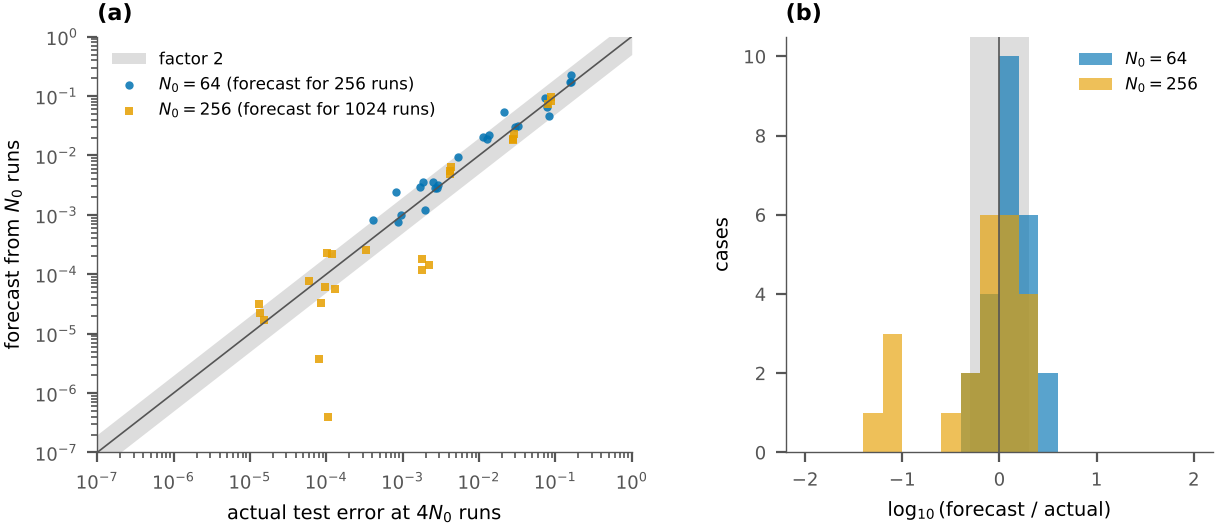
\includegraphics[width=\textwidth]{figures/fig_validity.png}
\caption{The learning-curve forecast is useful from small budgets and too optimistic from larger ones. (a) Forecast against actual test error at four times the starting budget (48 cases; problems solved by third-party code; shaded: within a factor two). (b) Histogram of $\log_{10}$(forecast/actual); cases below $-0.3$ are forecasts that are too low.}\label{fig:validity}\end{figure}
\paragraph{Basis check (H3)} The flag was raised in \HthreeJobs{} of the 72 fits, which are \HthreeCells{} distinct (problem, budget) cells from \HthreeProblems{} problems (convection--diffusion and transient heat); in all of them a full-field Gaussian process had a test error more than 10\% below the best POD-based member (H3 \FoneVerdict; the comparison is by test error over five POD members and two full-field members). This evidence is thinner than the count suggests. The flag was raised in only \HthreeRecall{} of the \HthreeFullJobs{} fits in which a full-field member was better by more than 10\%, so its recall is low, and in all \HthreeSelected{} flagged fits the cross-validated selection had already chosen a full-field member, so on these data the flag explained a decision rather than changed it. The flagged problems are those where the benchmark found networks competitive with the POD-based Gaussian process, which is consistent with Proposition 2.
\paragraph{Against a tuned network (H4)} The tuned network (Optuna, 16 trials; compared with the benchmark networks it also has four times the epochs, double precision and an L-BFGS polish, and about twice the trials) was better than the tool-selected model by more than 25\% in \SfourBetter{} of \SfourN{} cells (H4 \SfourVerdict, exactly at the limit of four). These \SfourBetter{} cells come from \StrongProblemsN{} problems (composite conduction and the L-shaped plate, both with seven or nine inputs, at two budgets each), and the Wilson interval for their share, \SfourWlo--\SfourWhi, is wide. The median ratio of the tool's error to the tuned network's was \SfourMedian; the tool was better by more than 10\% in \SfourToolBetter{} cells and the network in \SfourStrongBetter. The tuned network improved on the benchmark's networks in \StrongLegacyN{} of 16 cells (median error ratio \StrongLegacyRatio), but on the smooth problems at $N=1024$ its error was still up to \StrongWorstProblemRatio{} times that of the tool, so it is probably under-trained and H4 says little about what a well-tuned network could reach. It needed a median of \StrongSecTwofiftysix{}~s ($N=256$) and \StrongSecTentwentyfour{}~s ($N=1024$) on one core, against \ToolFitSecTwofiftysix{} and \ToolFitSecTentwentyfour{}~s for the tool's cross-validated selection (Section 6.4).
\begin{figure}[t]\centering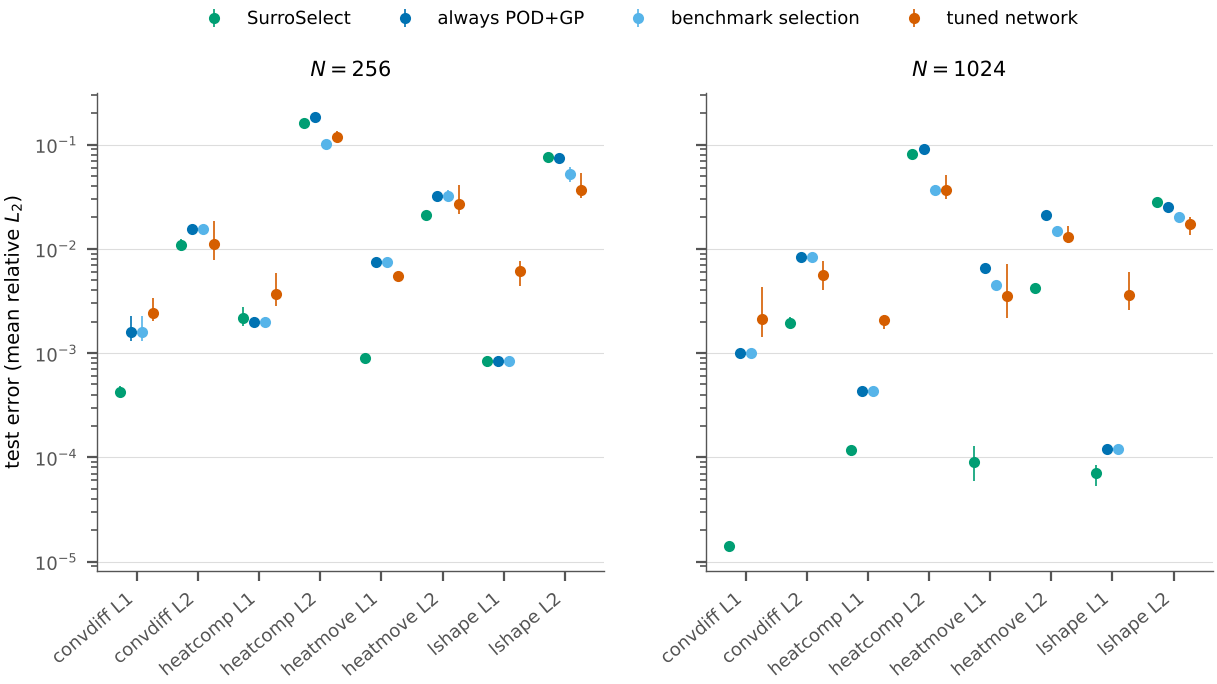
\includegraphics[width=\textwidth]{figures/fig_strong_nn.png}
\caption{Test error of the tool and its competitors on each problem solved by third-party code. Points: geometric mean over three seeds; bars: minimum to maximum over seeds. The tuned network was run at $N=256$ and $1024$ only.}\label{fig:strong}\end{figure}
The tool's advantage over the tuned network is largest on the smooth problems, and the network wins on the two problems with seven or nine inputs (Fig. 5).

\subsection{Ablation, noise and cost}\label{sec:cost}
\paragraph{Ablation} Restricting the pool, with selection by the stored cross-validation errors (Table 6), shows which members matter: without the full-field Gaussian process the regret is within a factor two in only \AblPodonlyShare{} of cells, and without any Gaussian-process member (ridge and polynomial only) the test error is a median \AblNogpMedian{} times larger than with the full pool.
\begin{table}[t]\centering\caption{Ablation of the pool on the eight problems solved by third-party code (24 cells); regret as in Section 5.}\label{tab:ablation}\small\resizebox{\textwidth}{!}{\begin{tabular}{lrrr}
\toprule
Pool & Median regret & Cells with regret $\le2$ & Median error vs full pool \\
\midrule
full pool & 1.00 & 100\% & 1.00$\times$ \\
POD-based members only & 1.07 & 75\% & 1.02$\times$ \\
no full-field GP & 1.07 & 75\% & 1.02$\times$ \\
GP members only & 1.01 & 96\% & 1.00$\times$ \\
no GP (ridge, polynomial) & 2.81 & 33\% & 2.74$\times$ \\
\bottomrule
\end{tabular}
}\end{table}
\paragraph{Sampling noise} A pool member picked at random gives median regret \NullRegret, and the seed-to-seed spread of the tool's regret is small (median regret \SoneMedianSixtyfour, \SoneMedianTwofiftysix{} and \SoneMedianTentwentyfour{} at the three budgets), so the observed regrets are not explained by chance. Seeds share the pool and test set and nest their training subsets, so seed variability understates the variability of a new sample of runs.
\paragraph{Computational cost} Measured on \HwCores{} cores (\HwCpu), one thread per fit, selection with cross-validation took a median of \ToolFitSecSixtyfour{}, \ToolFitSecTwofiftysix{} and \ToolFitSecTentwentyfour{}~s at $N=64$, 256 and 1024; adding the learning curve brought this to \ToolTotalSecSixtyfour{}, \ToolTotalSecTwofiftysix{} and \ToolTotalSecTentwentyfour{}~s. The solvers of these problems take \TpFomLo--\TpFomHi~ms per run, so for them the tool costs more than running the simulation 1024 times; its use is justified when one run takes minutes or hours.
\paragraph{Complexity} Let $N$ be the number of runs, $m$ the number of outputs, $p$ the number of inputs, $r$ the number of POD modes and $k$ the number of folds. The dominant costs are: an exact Gaussian process with fixed hyper-parameters, $O(N^3+N^2 r)$ per fit; hyper-parameter fitting, which uses at most 300 runs and costs $O(n_{\rm opt}^3 p)$ per optimiser step on the leading modes; kernel ridge, one eigendecomposition per kernel and length-scale, $O(N^3)$ each, with the whole ridge grid scored in $O(N^2)$ each; the polynomial, one singular value decomposition of the $N\times F$ design matrix with $F\le3000$, $O(NF^2)$; the full-field Gaussian process, as the POD-based one with all $m$ outputs sharing one kernel, $O(N^3+N^2m)$; the POD, $O(Nm\min(N,m))$. Cross-validation multiplies each by $k$, and the learning curve adds about $\sum_j k\,c(N/2^j)$, i.e.\ roughly one further cross-validated fit of the selected member. Between $N=256$ and $1024$ the measured median selection time grew by a factor of about \ToolScaleRatio, against the factor 64 predicted by cubic scaling, because the hyper-parameter fit is capped at 300 runs.

\subsection{Qualitative analysis}\label{sec:qualitative}
Fig. 6 shows the first test sample in dataset order for the first problem of each family at $N=256$ (seed 0), and failure cases selected by rules fixed before the figure was made: the problem with the largest selection regret at $N=256$ and the problem with the largest test error (a problem that is already shown is not repeated). The selected model reproduces the large-scale structure of the fields in the rule-selected examples, with relative errors given beside each panel; the error maps show structure rather than noise, so the remaining error is systematic. In the failure case with the largest error (the nine-input, high-contrast composite-conduction problem) the error is spread over the whole field, so no member of the pool captures this map at 256 runs; this is consistent with the benchmark, where networks beat the reduced-basis group on this problem.
\begin{figure}[t]\centering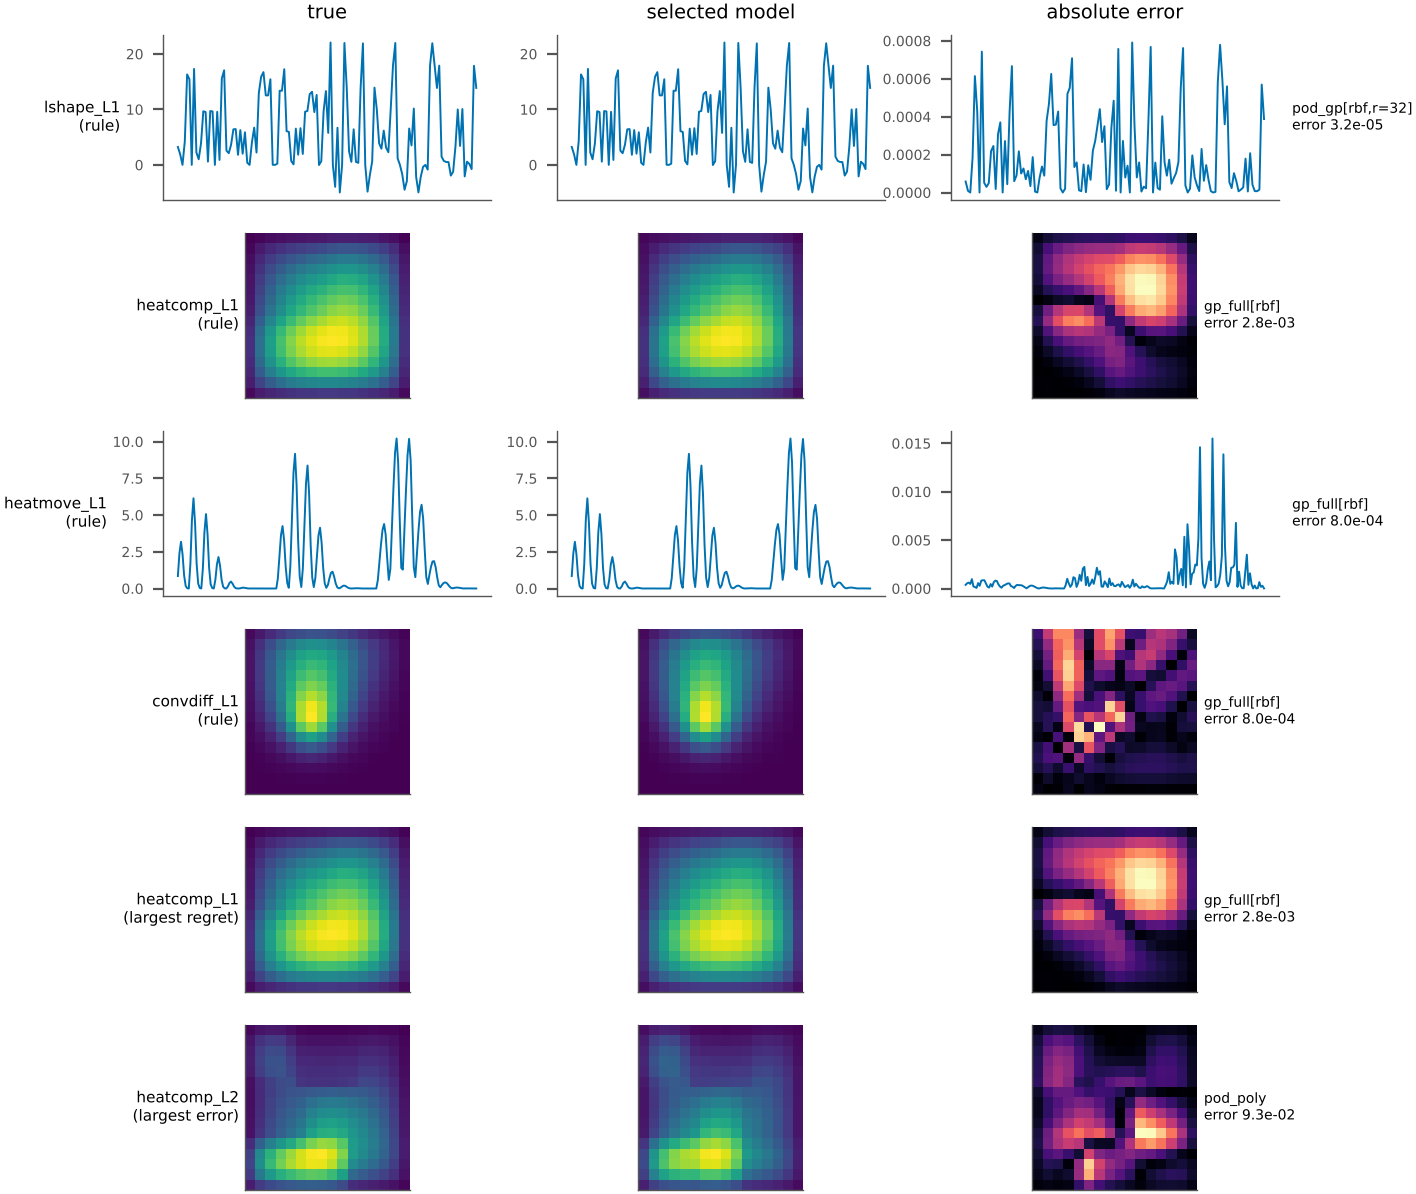
\includegraphics[width=0.9\textwidth]{figures/fig_qualitative.png}
\caption{The selected model reproduces the large-scale structure of single test fields; its errors are systematic. Predictions of the selected model on single test samples chosen by a fixed rule (first test sample in dataset order, first problem of each family, plus the failure cases defined in Section 6.5). Columns: true field, selected model, absolute error; the L-shaped plate has no regular grid and is shown as a profile over probe nodes.}\label{fig:qual}\end{figure}

\subsection{Comparative analysis and real-data check}\label{sec:real}
\paragraph{Comparison with the benchmark} Together with Section 6.1: on smooth problems with few inputs a Gaussian-process or well-regularised kernel member of the pool is hard to beat; where the POD basis limits accuracy a full-field Gaussian process is the better choice; and where networks from the benchmark win (the composite-conduction problem with nine inputs), the default pool cannot match them (H1c). The tool's contribution is to find these cases from the training runs alone. In a descriptive, design-informed run on the 36 earlier problems (one seed, $N=256$; Supplement, Sec.~S7), the tool's selection can be compared with the oracle, but those problems were used to design the pool and the run is not evidence for the criteria.
\paragraph{Real measured data} Two real datasets were used (\texttt{data\_real/}, CC BY 4.0): wind-tunnel measurements of airfoil noise (1,503 rows, five inputs) and the output of a combined-cycle power plant (9,568 rows, four inputs). Both have a scalar, noisy output, so they violate assumption A2, are not field data, and make the POD rank one, so the data say nothing about the POD-versus-full-field choice that the tool is built around; the normalised RMSE replaces the relative error. With the protocol of Supplement addendum v3.1 (committed before any model was fitted to these data), median regret was \RealRoneMedian{} over six cells (R1 \RealRoneVerdict), the tool was no worse than always-POD+GP in \RealRtwoK{} of \RealRtwoN{} cells (R2 \RealRtwoVerdict; two of the successes are exact ties, because the same model was chosen), the tuned network was better by more than 25\% in \RealRthreeK{} cells (R3 \RealRthreeVerdict), and \RealRfourK{} of \RealRfourN{} forecasts were within a factor two (R4 \RealRfourVerdict). We had predicted that R4 would fail because of measurement noise; it did not. The airfoil pool holds only 1,052 rows, so its $N=1024$ results use nearly all of it. Table 7 lists the errors.
\begin{table}[t]\centering\caption{Real-data check: normalised RMSE of the tool, the oracle, always-POD+GP and the tuned network (geometric mean over three seeds).}\label{tab:real}\small\resizebox{\textwidth}{!}{\begin{tabular}{lrrrrrr}
\toprule
Dataset & N & Tool & Oracle & Always GP & Tuned net & Regret \\
\midrule
airfoil & 64 & 0.5960 & 0.5218 & 0.5868 & 0.6792 & 1.14 \\
airfoil & 256 & 0.3585 & 0.3578 & 0.3585 & 0.4072 & 1.00 \\
airfoil & 1024 & 0.2107 & 0.1845 & 0.2107 & 0.2037 & 1.14 \\
ccpp & 64 & 0.2867 & 0.2676 & 0.3153 & 0.5854 & 1.07 \\
ccpp & 256 & 0.2554 & 0.2539 & 0.2920 & 0.3682 & 1.01 \\
ccpp & 1024 & 0.2453 & 0.2437 & 0.2500 & 0.3530 & 1.01 \\
\bottomrule
\end{tabular}
}\end{table}
\paragraph{Plain-file validation and case study} The three command-line commands were run on exported files for three problems; all sequences ran, and the error printed by \texttt{evaluate} matched an independent computation (Supplement, Sec.~S8). 7 shows the report for problem \texttt{heatmove\_L1} with 256 runs and a target error of 0.1\%.
\begin{figure}[t]\centering\small
\begin{minipage}{0.95\textwidth}\scriptsize\verbatiminput{tables/case_report_wrapped.txt}\end{minipage}
\caption{SurroSelect report (in Markdown) for \texttt{heatmove\_L1} (256 runs, seed 0, target error 0.1\%), unedited except for line wrapping.}\label{lst:case}\end{figure}

\section{Discussion}\label{sec:discussion}
\paragraph{What the evidence supports} On the problems solved by third-party code, cross-validated selection from a small pool of classical models found the oracle or a near-oracle member (H1a; a fixed choice of one full-field Gaussian process does almost as well), was not worse than always using a Gaussian process (H1b; nearly guaranteed because that model is in the pool), raised the basis flag only in cases where a full-field model was better but with low recall (H3), and gave usable forecasts of the error at four times the budget when starting from 64 runs (H2). Against a tuned network the tool met the criterion of H4 only at its limit, and that network is probably under-trained. On real measured data with scalar, noisy outputs, all four descriptive criteria were met.
\paragraph{What it does not support} The benchmark finding that the reduced-basis group wins at large budgets did \emph{not} hold on \TpNotClear{} of the \TpN{} problems (H5 \TpVerdict), so a fixed recommendation ``use a reduced-basis Gaussian process'' is not safe; the case for the tool is that it finds out from the data. The tool did not match the benchmark's own selection among five methods that include networks (H1c \SthreeVerdict): where networks win, the default pool, which has none, loses. The forecast was too optimistic from 256 runs, and its range is not an uncertainty interval. We did not isolate marginal-likelihood fitting as the mechanism behind the Gaussian-process advantage, and the pilot diagnostic that we had hoped would predict the winner from 32 runs was not confirmed (Supplement, Sec.~S3).
\paragraph{Limitations}
\begin{enumerate}
\item \textbf{Simulated problems.} All \NAllProblems{} problems are simulated; the eight problems solved by third-party code come from four families (two levels each) of one finite-element library. The real-data check uses two datasets with scalar, noisy outputs, which violate assumption A2; it says that the tool behaves sensibly on them, not that it works for noisy field data.
\item \textbf{Design knowledge.} The pool, the kernel-ridge grids and the criteria were designed with knowledge of the 36 earlier problems, so the problems solved by third-party code are out-of-sample only in part, and they were chosen by us after the earlier results were known, so ``independent'' refers to the solver, not to the choice of problems. Smoke tests of the tool on three of the eight problems preceded the commit of the criteria; they showed test errors of some pool members and exposed a numerical bug in the leave-one-out computation, which was fixed before the evaluation runs (deviation V9). The text of the criteria was not changed afterwards, but its statement that no error had been seen was wrong when written.
\item \textbf{Few independent units.} Cells within a problem are not independent, so the intervals in Table 4, which treat 24 cells as independent, are optimistic. Seeds share the pool and test set and nest their training subsets.
\item \textbf{Forecast.} The forecast is a power-law extrapolation without guarantee; it was too low by more than a factor two in \BoneUnder{} of \BoneN{} cases, and the pre-specified criterion was met with a confidence interval that includes the threshold.
\item \textbf{Networks.} The default pool contains no network. The tuned network uses 16 trials in a restricted space (depth 2--4, width 64--256) on one core; a more heavily tuned or different architecture could do better.
\item \textbf{Cost.} The solvers take milliseconds per run, so on these problems the tool costs more than the simulations it replaces; its use is justified for much slower simulations, which we did not test.
\item \textbf{Scope of the tool.} It assumes exchangeable runs on a common output grid, deterministic outputs, and a moderate number of inputs (only \NHighP{} of our \NAllProblems{} problems have ten or more).
\item \textbf{Process.} Hypotheses and code were committed before the runs they concern, but the history is our own, not an independent registry; several stages were designed after seeing earlier results (labelled post hoc); the independent reviews were performed by AI agents, not human reviewers.
\end{enumerate}
\paragraph{Ethics and disclosure} No human or animal subjects were involved. The two real datasets are public (CC BY 4.0). The AI involvement is disclosed in the acknowledgments.



\section{Conclusion and Future Scope}\label{sec:conclusion}
We built SurroSelect, a procedure and open tool that chooses a stand-in for a slow simulation by cross-validation, reports ties, checks whether the POD basis limits accuracy and forecasts the error for more runs, and we tested it against criteria committed in advance on eight problems solved by an independent finite-element library. Selection was within a factor \SoneMax{} of the oracle (the best pool member) in all 24 cells, although one fixed full-field Gaussian process does almost as well; the basis check raised a flag only in cases where a full-field model was better, but missed most such cases; the tool did not beat the benchmark's selection among networks and Gaussian-process variants, and its forecast was usable from small budgets only. A 44-problem study showed that the winner depends on smoothness, the number of inputs, the budget, the training effort of the networks and how widely a kernel method's regularisation is searched, and that the simple rule ``reduced basis wins at large budgets'' fails on \TpNotClear{} of \TpN{} problems solved by third-party code.
Concrete next steps are (i) a pool that includes a tuned network, with a rule for when to spend its cost; (ii) a forecast that models the error floor and gives a calibrated interval; (iii) tests on real field data from simulations that are much slower than ours, with the full cost of the simulations included; (iv) a public benchmark such as PDEBench~\cite{takamoto2022}; and (v) independent human replication.

\section*{Acknowledgments}
\textbf{Use of AI tools.} The study design, code, analyses, figures and the drafting of this paper were carried out with an AI system (Claude, Anthropic) acting as a research assistant under the authors' direction. The internal ``reviews'' and audits mentioned in the supplement were performed by AI agents, not by human reviewers. The authors are responsible for the content, have checked it (to be confirmed by the authors before submission), and all authors must approve the submission. [Funding, other acknowledgments and competing-interest statement: to be supplied by the authors.]

\section*{Data and code availability}
All data are generated by the code in the project repository from problem names and seeds; raw outputs, aggregation scripts (which write every number in this paper) and figure scripts are included, and \texttt{code/run\_all.py} reruns everything. The tool is the \texttt{surroselect} package (MIT licence; copyright holder to be set by the authors). A permanent archive with a DOI has not been created yet: [authors to provide the public repository link or archive DOI before submission].

\bibliographystyle{elsarticle-num}
\bibliography{references}
\end{document}
